% ARCHITECTURE
\chapter{Architecture}\label{chapter:architecture}

% General architecture of the application
% central server with API and three mobile apps
% MVC REST API to mobile App
% MVC in the App's internal structure

\section{Data model}\label{section:datamodel}

Figure \ref{figure:erd} shows the entity relationship diagram (ERD) of the entities in the database.

\begin{figure}
	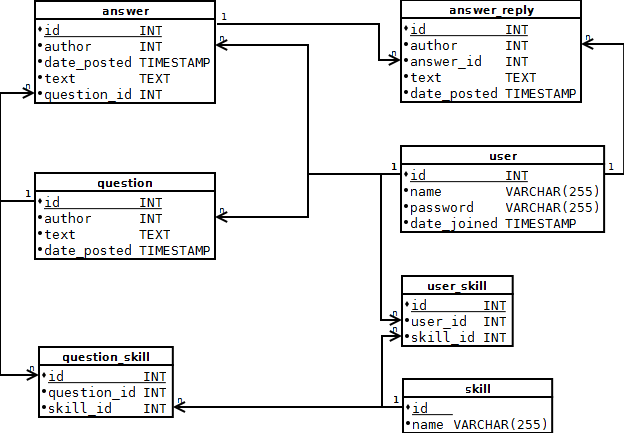
\includegraphics[width=400px]{img/erd}
	\caption{Entity relationship diagram of the database.}
	\label{figure:erd}
\end{figure}



\section{REST API}\label{section:restapi}

To allow access to the database, each application can talk to a public interface. The REST API consists out of a series of methods, listed in table \ref{table:rest_api}. The parameter names of the returned data are based on the database table and column names.

% REFERENCE ... wikipedia, tutorial


\begin{table}
	\caption{REST API}
	
	\begin{center}
		\begin{tabular}{p{70px} | p{70px} | p{210px}}
				\hline
				\hline
				\textbf{Resource} 		& \textbf{Method}					&	\textbf{Description} 	\\
				\hline
				\hline
				\texttt{USER}					&	\\
				\hline
															& \emph{get\_info}				&	Retrieve profile information about a user.	\\
															& \emph{update\_info}			& Update profile information about a user. \\
															& \emph{get\_questions}		& Get questions submitted by a user. \\
															& \emph{register}					&	Register a new user account. \\
															& \emph{delete}						&	Delete a user account. \\
															& \emph{search}						&	Search a user given certain parameters. \\
															& \emph{get\_skills}			& Get the skills of a user. \\
															& \emph{get\_answers}			& Get the answers submitted by a user. \\
															%& \emph{getContacts}	  	& \\
															%& \emph{}									& \\
				\hline
				\texttt{SKILL}				& 												& \\
				\hline
															& \emph{search}						& Search skills. \\
															& \emph{create}						& Create a new skill and add it to the database. \\
															& \emph{get\_questions}		& Get questions related to a given skill. \\
				\hline
				\texttt{QUESTION}			& 												& \\
				\hline
															& \emph{search}						& Search questions, given a number of search parameters. \\
															& \emph{get\_answers}			& Get the answers for a question. \\
															& \emph{get\_skills}			& Get the skills related to this question. \\
															& \emph{create}						& Post a new question. \\
															& \emph{get\_info}				& Get information on a question. \\
															& \emph{delete}						& Delete a question. \\
				\hline
				\texttt{ANSWER}				& 												&	\\
				\hline
															& \emph{search}						& Search an answer.	\\
															& \emph{get\_question}		& Get the question this answer was posted on. \\
															& \emph{create}						& Create a new answer. \\
				\hline
				\hline
		\end{tabular}
	\end{center}

	\label{table:rest_api}
\end{table}
